% !TEX root = main.tex
\section{Flavour Tagging}
\label{sec:Tagging}
To successfully perform a time- and amplitude-dependent measurement of $\gamma$, the identification of the initial state flavour of the $\Bs$ meson is crucial.
In the presented analysis, a number of flavour tagging algorithms are used that either determine the flavour of the non-signal b-hadron produced in the event (opposite site, OS), 
or they use particles produced in the fragmentation of the signal candidate $\Bs$/$\Bsb$ (same side, SS). \newline
For the same side, the algorithm searching for the charge of an aditional kaon that acompanies the fragmentation of the signal candidate is used (SS-nnetKaon). For the opposite site, four different taggers are chosen: 
The Two algorithms that use the charge of an electron or a muon from semileptonic B decays (OS- $\electron$,$\muon$), the tagger that uses the charge of a kaon from a b $\to$ c $\to$ s decay chain (OS-nnetKaon) 
and the algorithm that determines the $\Bs$/$\Bsb$ candidate flavour from the charge of a secondary vertex, reconstructed from the OS b decay product (OS-VtxCharge). 
All four taggers are then combined into a signel OS tagger. \newline
Every single tagging algorithm is prone to misidentify the signal candidate at a certain mistag rate $\omega = (wrong tags)/ (all tags)$. 
This might be caused by particle misidentification, flavour oscillation of the neutral opposite site B-meson or by tracks that are wrongly picked up from the underlying event. 
For every signal $\Bs$/$\Bsb$ candidate, each tagging algorithm predicts a mistag probability $\eta$, which is calculated using a combination of inputs such as the kinematics of the tagging particles. 
The inputs are then combined to a predicted mistag using neural networks. These are trained on simulated samples of $\Bs\to\Dsm\pip$ (SS algorithm) and $\Bu\to\jpsi\Kp$ (OS algorithms) decays.
For the presented analysis, the measurable CP-violating coefficients are damped by the tagging dilution $D$, that depends on the mistag rate:

\begin{equation}
\label{eq: taggingDilution}
D = 1 - 2\omega.
\end{equation}

This means that the statistical precision, with which these coeffcients can be measured, scales as the inverse square root of the effective tagging efficiency,

\begin{equation}
\label{eq: taggingEfficiency}
\epsilon_{eff} = \epsilon_{tag}(1 - 2\omega)^{2},
\end{equation}

where $epsilon_{tag}$ is the fraction of events that have a tagging decision. 
The flavour tagging algorithms are optimised for highest $\epsilon_{eff}$ on data, using the $\Bs\to\Dsm\pip$ and $\Bu\to\jpsi\Kp$ samples. \newline
Utilizing flavour-specific final states, the predicted mistag $\eta$ of each tagger has to be calibrated to match the observed mistag $\omega$ on the data sample. 
For the calibration, a linear model of the form

\begin{equation}
\label{eq: mistagCalibration}
\omega(\eta) = p_{o} + p_{1} \cdot (\eta - < \eta >), 
\end{equation}  

where the values of $p_{0}$ and $p_{1}$ are determined using the $\Bs\to\Ds\pion\pion\pion$ normalization mode and $<\eta>$ is the average estimated mistag probability $<\eta> = \Sigma_{i=1}^{N_{cand}}(\eta_{i}) / N_{cand}$.
Following this model, a perfectly calibrated tagger would lead to $\omega(\eta) = \eta$ and one would expect $p_{1} = 1$ and $p_{0} = <\eta>$.
Due to the different interaction cross-sections of oppositely charged particles, the tagging calibration parameters depend on the initial state flavour of the $\Bs$. 
Therefore, the flavour asymmetry parameters $\Delta p_{0}$, $\Delta p_{1}$ and $\Delta\epsilon_{tag}$ are introduced. 
For this analysis, the calibrated mistag is treated as per-event variable, giving a larger weight to events that are less likely to have an incorrect tag. 
This adds one additional observable to the time- and amplitude-dependent fit. \newline
The tagging calibration is determined using a time-dependent fit to the full $\Bs\to\Ds\pion\pion\pion$ sample, where the mixing frequency $\dms$ is fixed to the nominal PDG value \cite{PDG2014}.
The calibration procedure for the OS tagging algorithms (Sec.\ref{subsec: OScalibration}) and 
the SS kaon tagger (Sec.\ref{subsec: SScalibration}) is applied on the full Run I and 2015 and 2016 Run II $\Bs\to\Ds\pion\pion\pion$ data sample, which is selected following the steps described in Sec. \ref{sec:Selection}.
The similar selection ensures as close as possible agreement between the $\Bs\to\Ds\pion\pion\pion$ and $\Bs\to\Ds\kaon\pion\pion$ samples in terms of the decay kinematics, which are crucial for the flavour tagging.
Section \ref{subsec: TaggingComparison} shows the compatibility of both samples. After applying the calibration, the response of the OS and SS taggers are combined, which is shown in Sec. \ref{subsec: TaggingCombination}.  




\subsection{OS tagging calibration}
\label{subsec: OScalibration}
The responses of the OS electron, muon, neural net kaon and the secondary vertex charge taggers are combined for the mistag calibration. 
Figure \ref{fig:OSdistribution} shows the distribution of the predicted OS mistag for signal candidates from $\Bs\to\Ds\pion\pion\pion$. 
The extracted calibration parameters and tagging asymmetries are summarized in Table \ref{table: OScalibration} and the measured tagging power for the OS combination is $\epsilon_{eff,OS} = 3.62 \%$.

\begin{figure}[h]
\centering
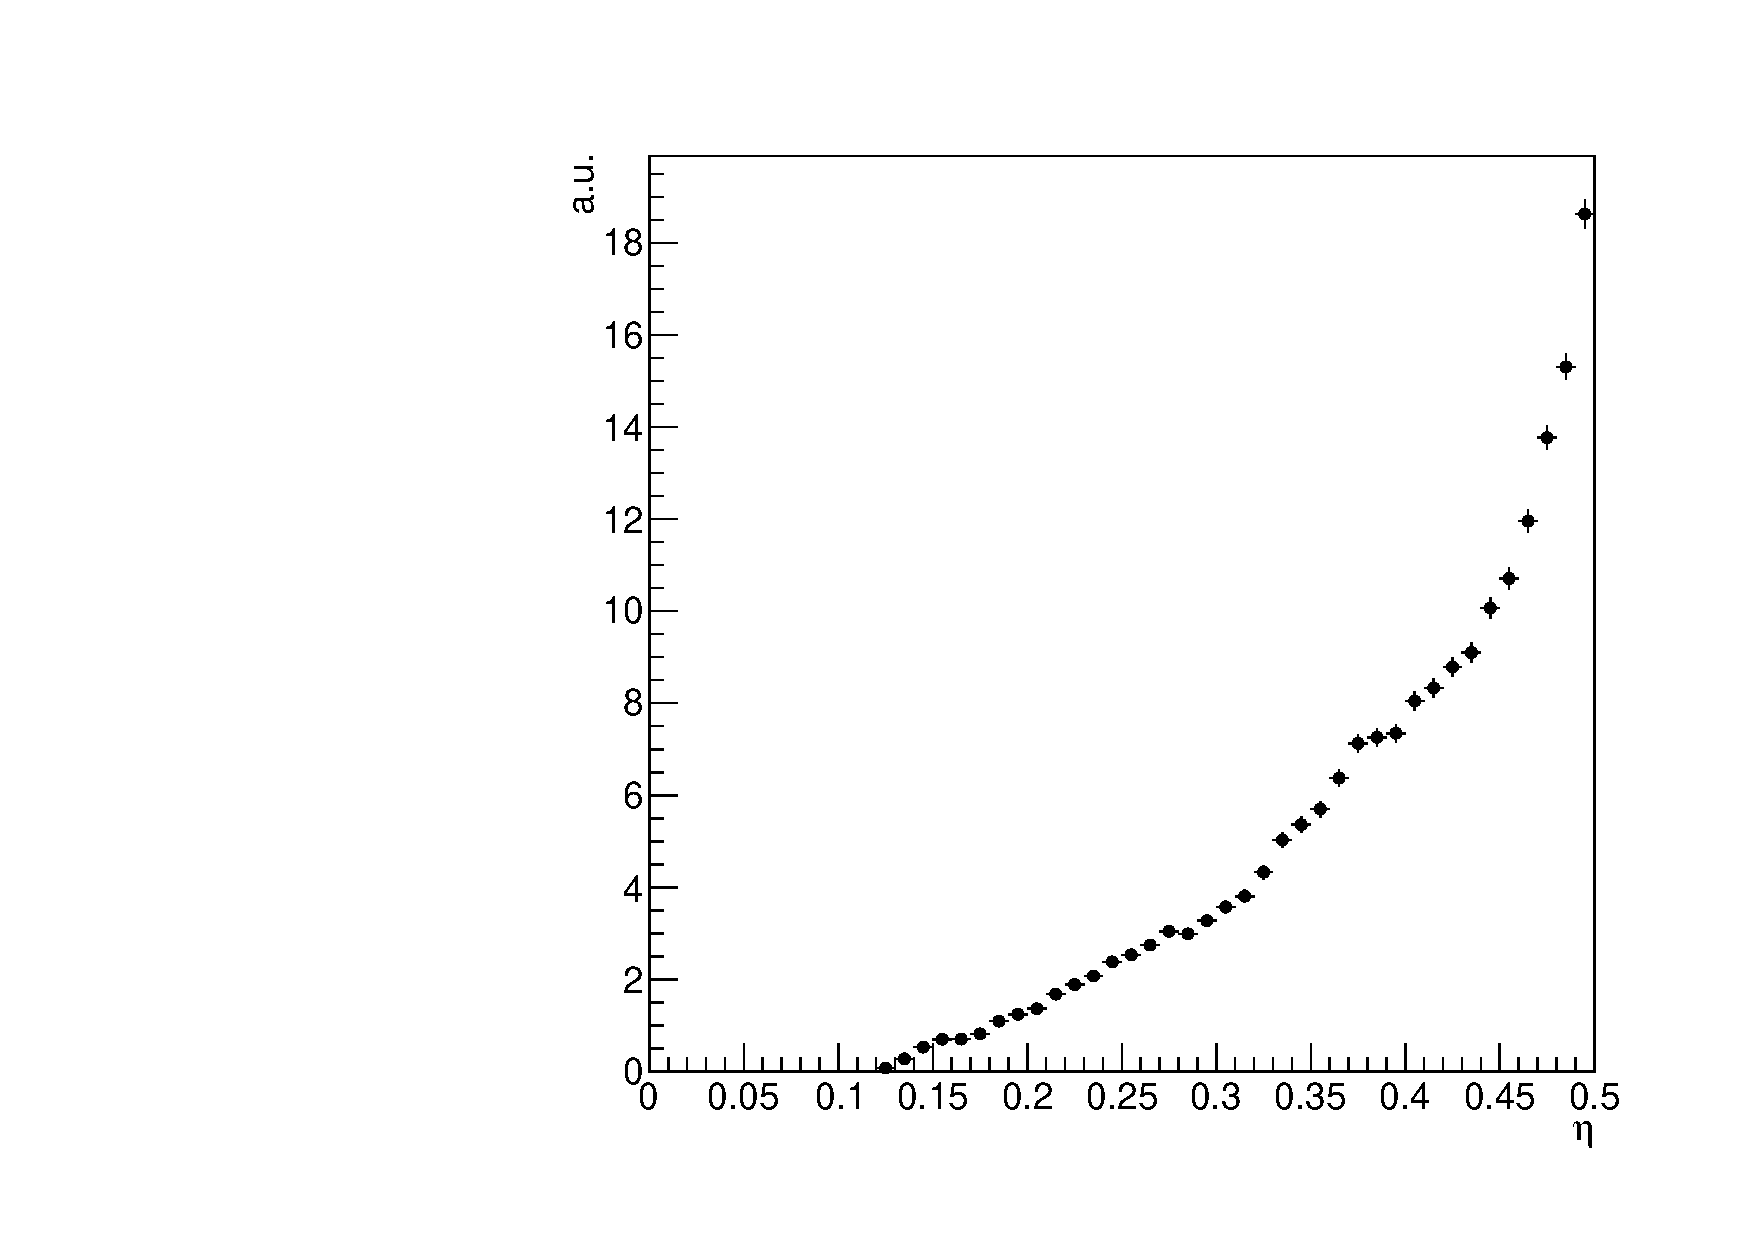
\includegraphics[height=7.4cm,width=0.7\textwidth]{figs/Tagging/OS_combination_etaDis.pdf}
\caption{Distribution of the predicted OS combination mistag probablity for $\Bs\to\Ds\pion\pion\pion$ signal candidates.}
\label{fig:OSdistribution}
\end{figure}


\begin{table}[h]
\centering
\scriptsize
 \begin{tabular}{l l l l | l l | l}
\hline
$p_{0}$ & $p_{1}$ & $<\eta>$ & $\epsilon_{tag}$ & $\Delta p_{o}$ & $\Delta p_{1}$ & $\epsilon_{eff}$ [$\%$] \\
\hline
0.039 $\pm$0.005  & 0.818 $\pm$ 0.042 & 0.370 & 0.517 $\pm$ 0.002 & 0.028 $\pm$ 0.005 & 0.037 $\pm$ 0.045 & 3.62 $\pm$ 0.03 (stat) $\pm$ 0.25 (cal) \\
\hline
\end{tabular}
\caption{Calibration parameters and tagging asymmetries of the OS tagger extracted from $\Bs\to\Ds\pion\pion\pion$ decays.}
\label{table: OScalibration}
\normalsize
\end{table}


\subsection{SS tagging calibration}
\label{subsec: SScalibration}
The SS neural net kaon tagger can be calibrated using the flavour-specific $\Bs\to\Ds\pion\pion\pion$ decay. It's development, performance and calibration is described in detail in \cite{Aaij:2016psi}. 
Figure \ref{fig:SSdistribution} shows the distribution of the predicted mistag of the neural net kaon tagger. 
The extracted calibration parameters and tagging asymmetries are summarized in Table \ref{table: SScalibration} and the measured tagging power for this algorithm is $\epsilon_{eff,SS} = 2.45  \%$.


\begin{figure}[h]
\centering
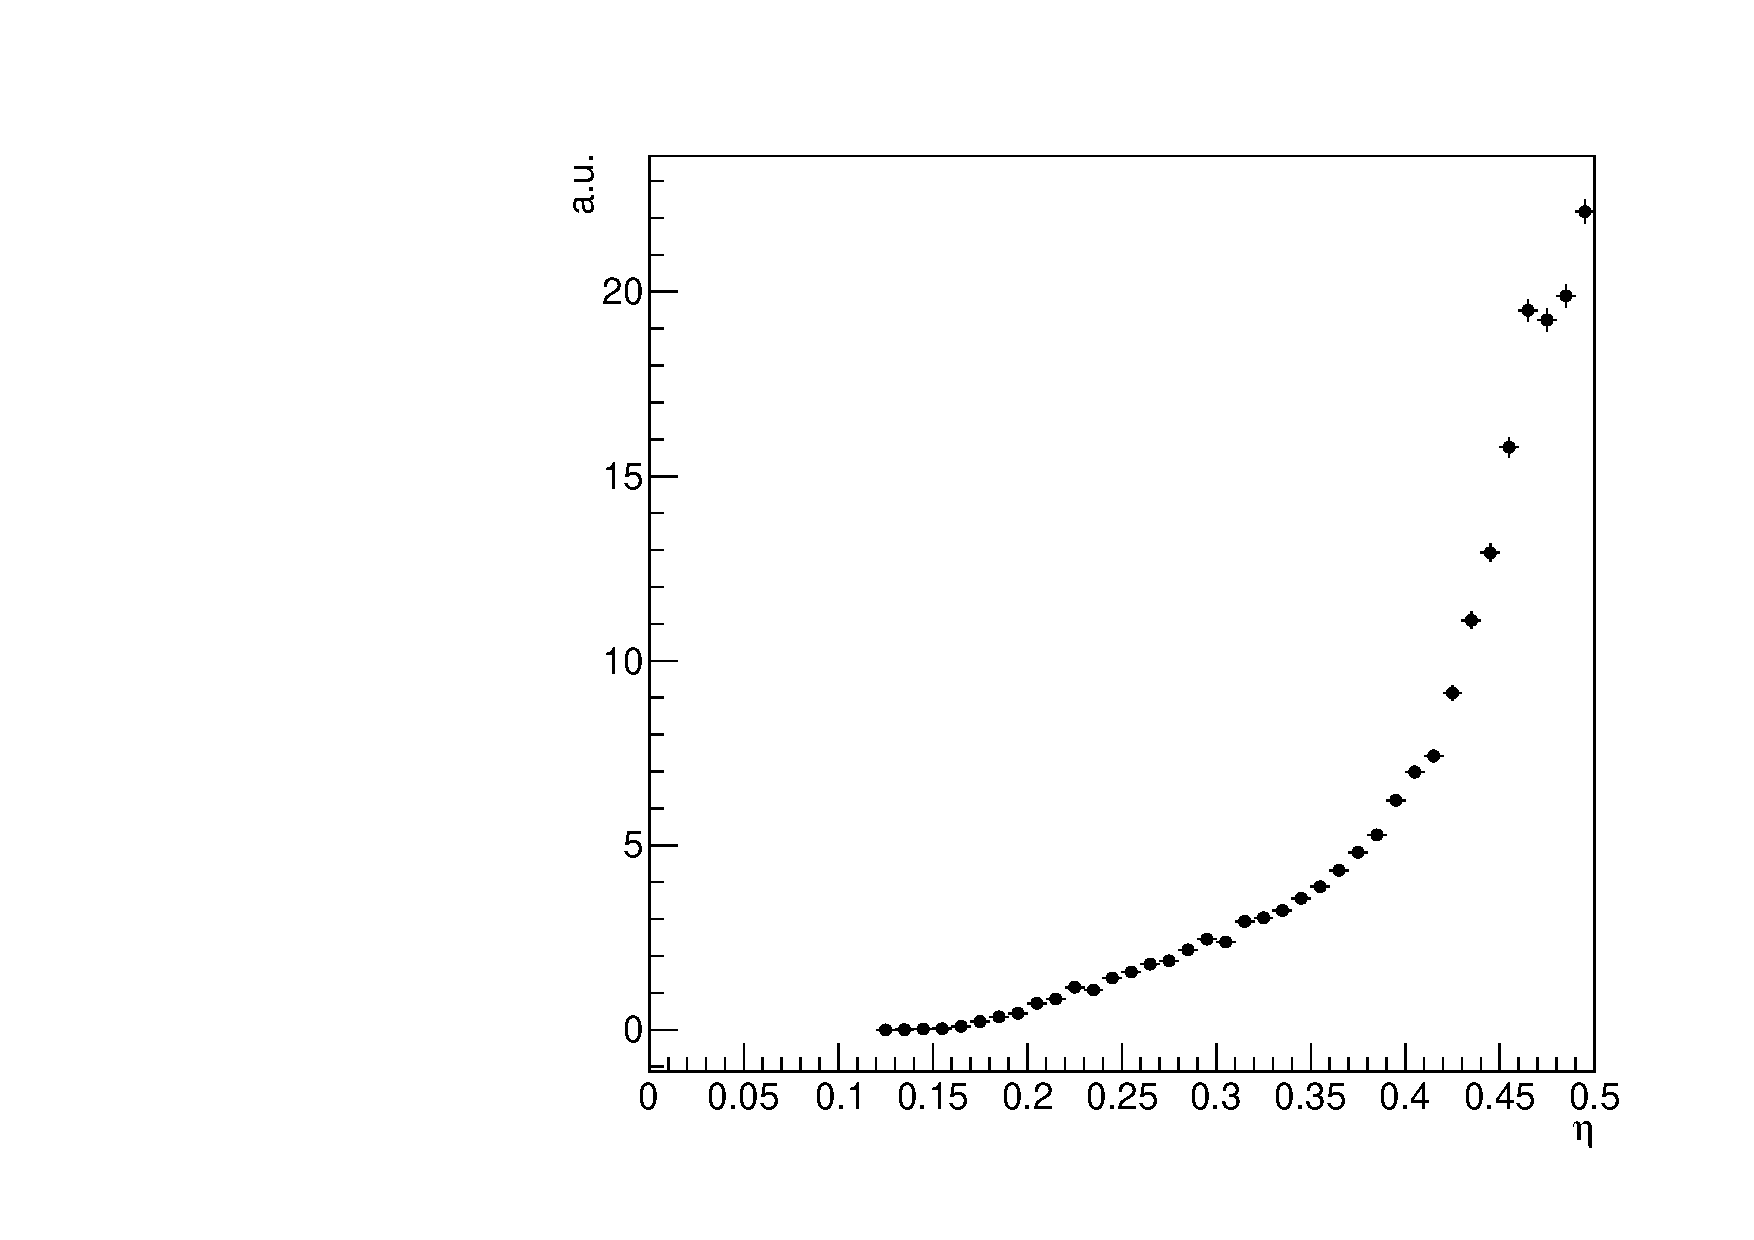
\includegraphics[height=7.4cm,width=0.7\textwidth]{figs/Tagging/SS_nnetKaon_etaDis.pdf}
\caption{Distribution of the predicted SS neural net kaon tagger mistag probablity for $\Bs\to\Ds\pion\pion\pion$ signal candidates.}
\label{fig:SSdistribution}
\end{figure}


\begin{table}[h]
\centering
\scriptsize
 \begin{tabular}{l l l l | l l | l}
\hline
$p_{0}$ & $p_{1}$ & $<\eta>$ & $\epsilon_{tag}$ & $\Delta p_{o}$ & $\Delta p_{1}$ & $\epsilon_{eff}$ [$\%$] \\
\hline
0.018 $\pm$ 0.004  & 0.948 $\pm$ 0.052 & 0.420 & 0.569 $\pm$ 0.002 & -0.017 $\pm$ 0.004  & 0.135 $\pm$ 0.058 & 2.45 $\pm$ 0.02 (stat) $\pm$ 0.20 (cal) \\
\hline
\end{tabular}
\caption{Calibration parameters and tagging asymmetries of the SS tagger extracted from $\Bs\to\Ds\pion\pion\pion$ decays.}
\label{table: SScalibration}
\normalsize
\end{table}


\subsection{Tagging performance comparison between the signal and normalization channel}
\label{subsec: TaggingComparison}

TO BE FILLED


\begin{figure}[h]
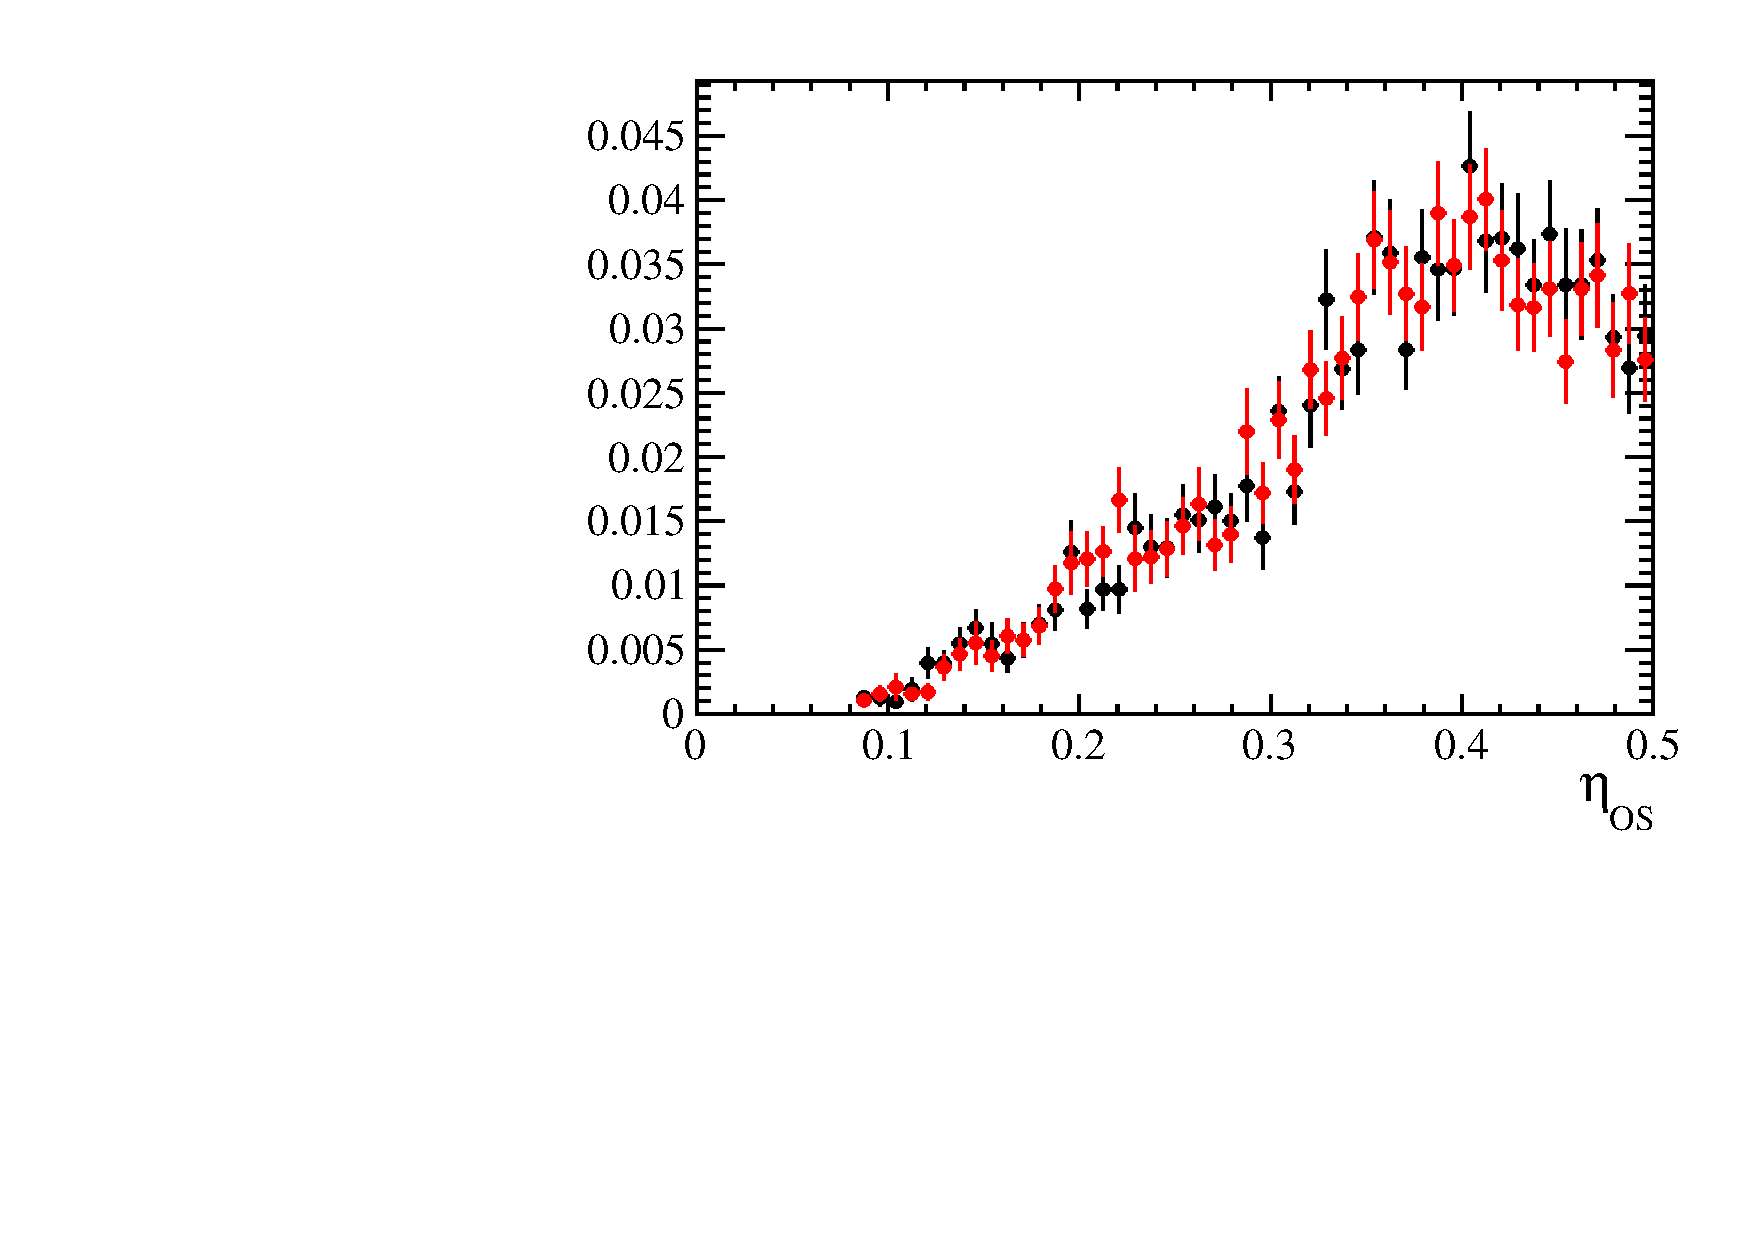
\includegraphics[height=7.cm,width=0.49\textwidth]{figs/Tagging/w_OS_MC.pdf}
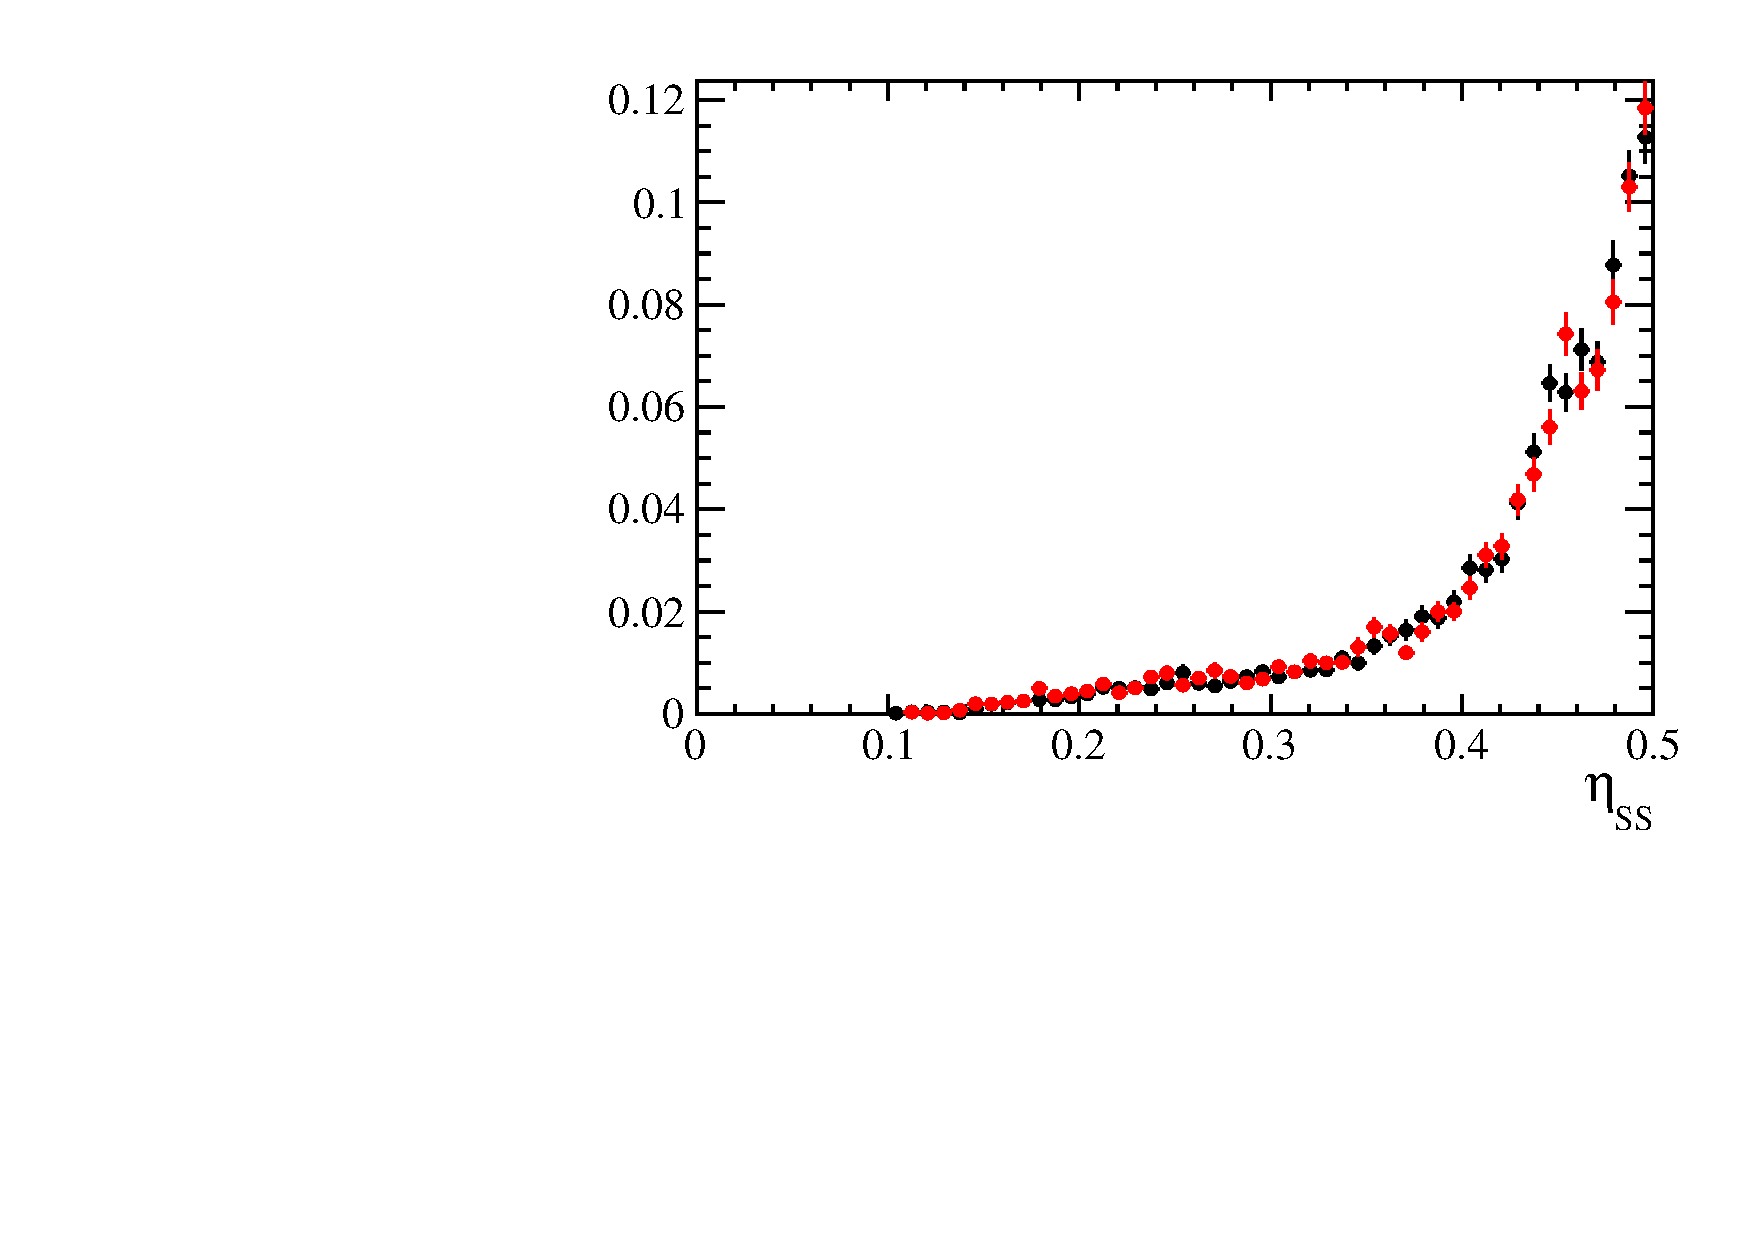
\includegraphics[height=7.cm,width=0.49\textwidth]{figs/Tagging/w_SS_MC.pdf}
\caption{Distributions of the predicted mistag $\eta$ for the OS combination (left) and the SS kaon tagger (right) in simulated $\Bs\to\Ds\kaon\pion\pion$ (black) and $\Bs\to\Ds\pion\pion\pion$ (red) signal.}
\label{fig:w_MC_comparison}
\end{figure}


\begin{figure}[h]
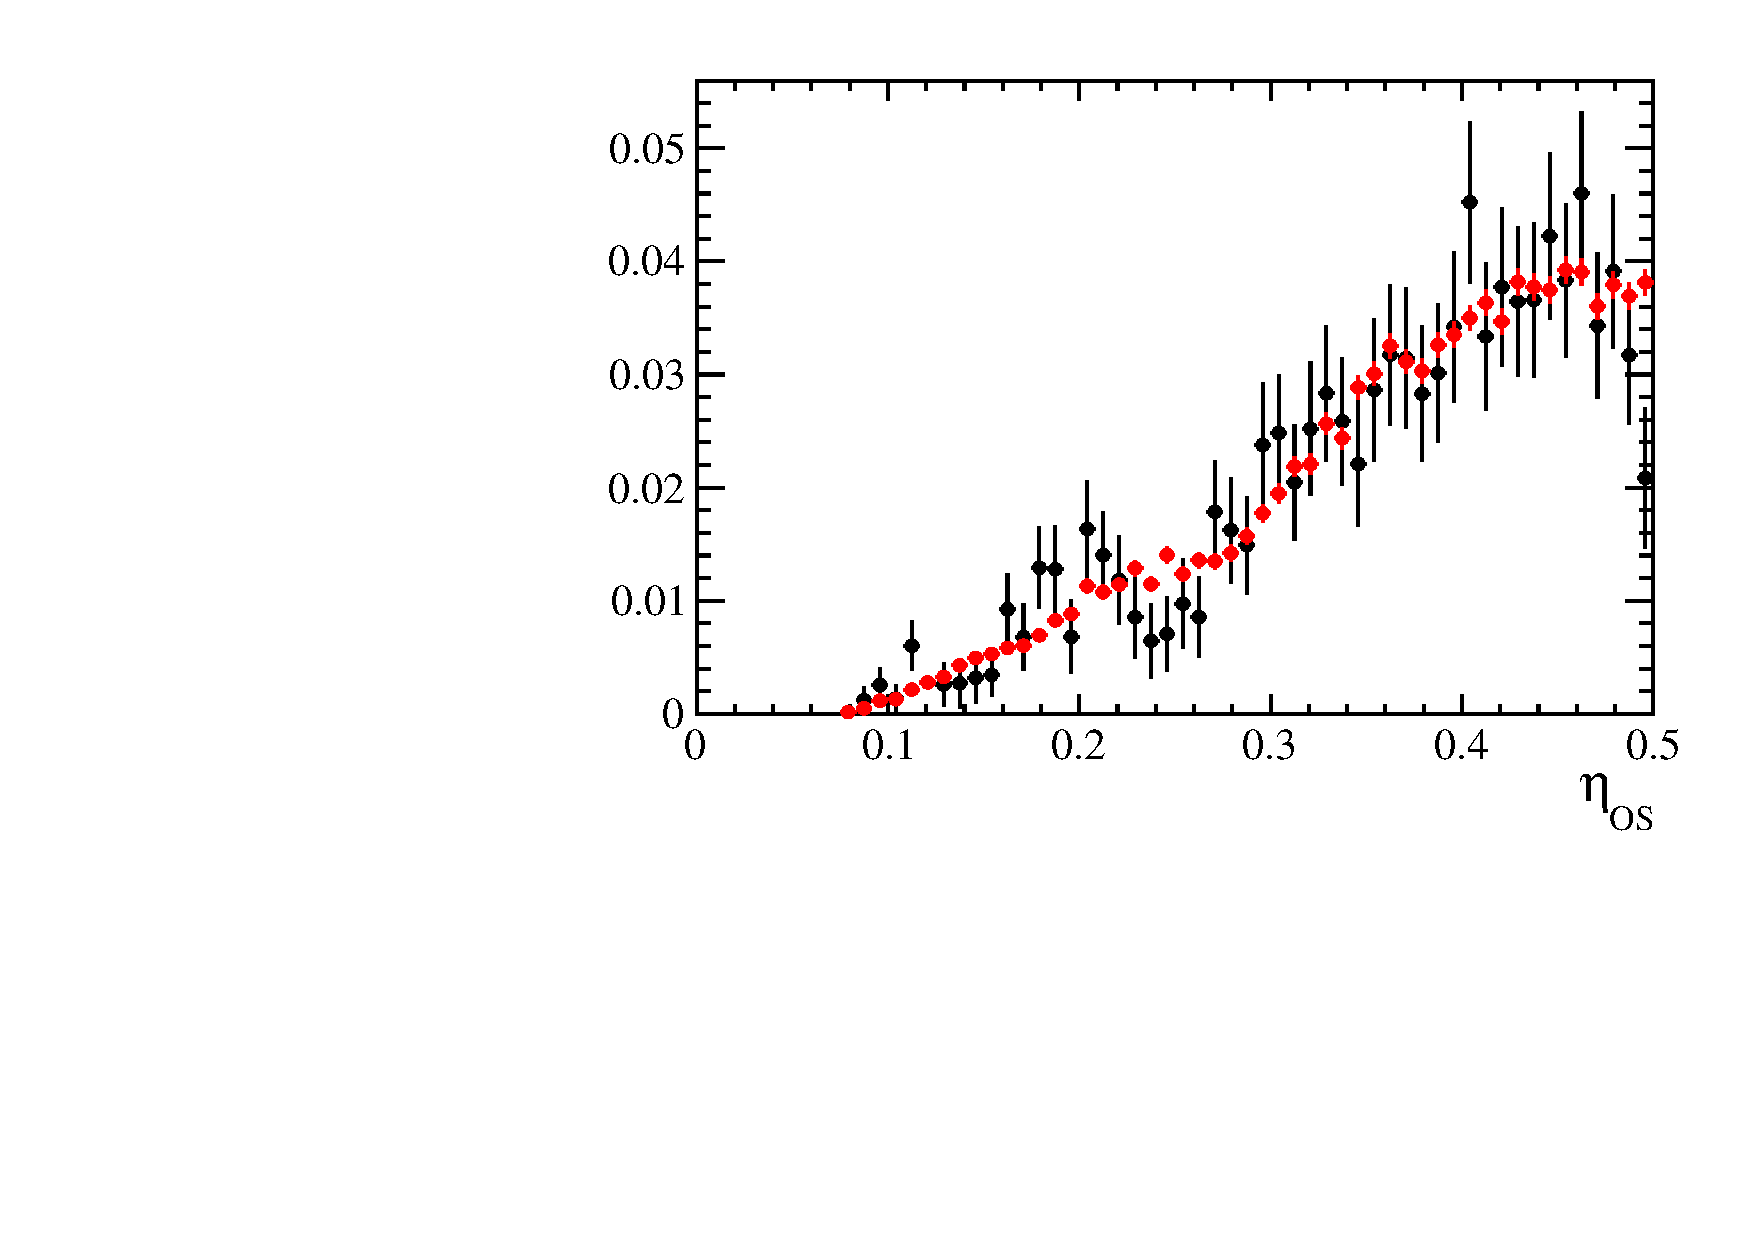
\includegraphics[height=7.cm,width=0.49\textwidth]{figs/Tagging/w_OS.pdf}
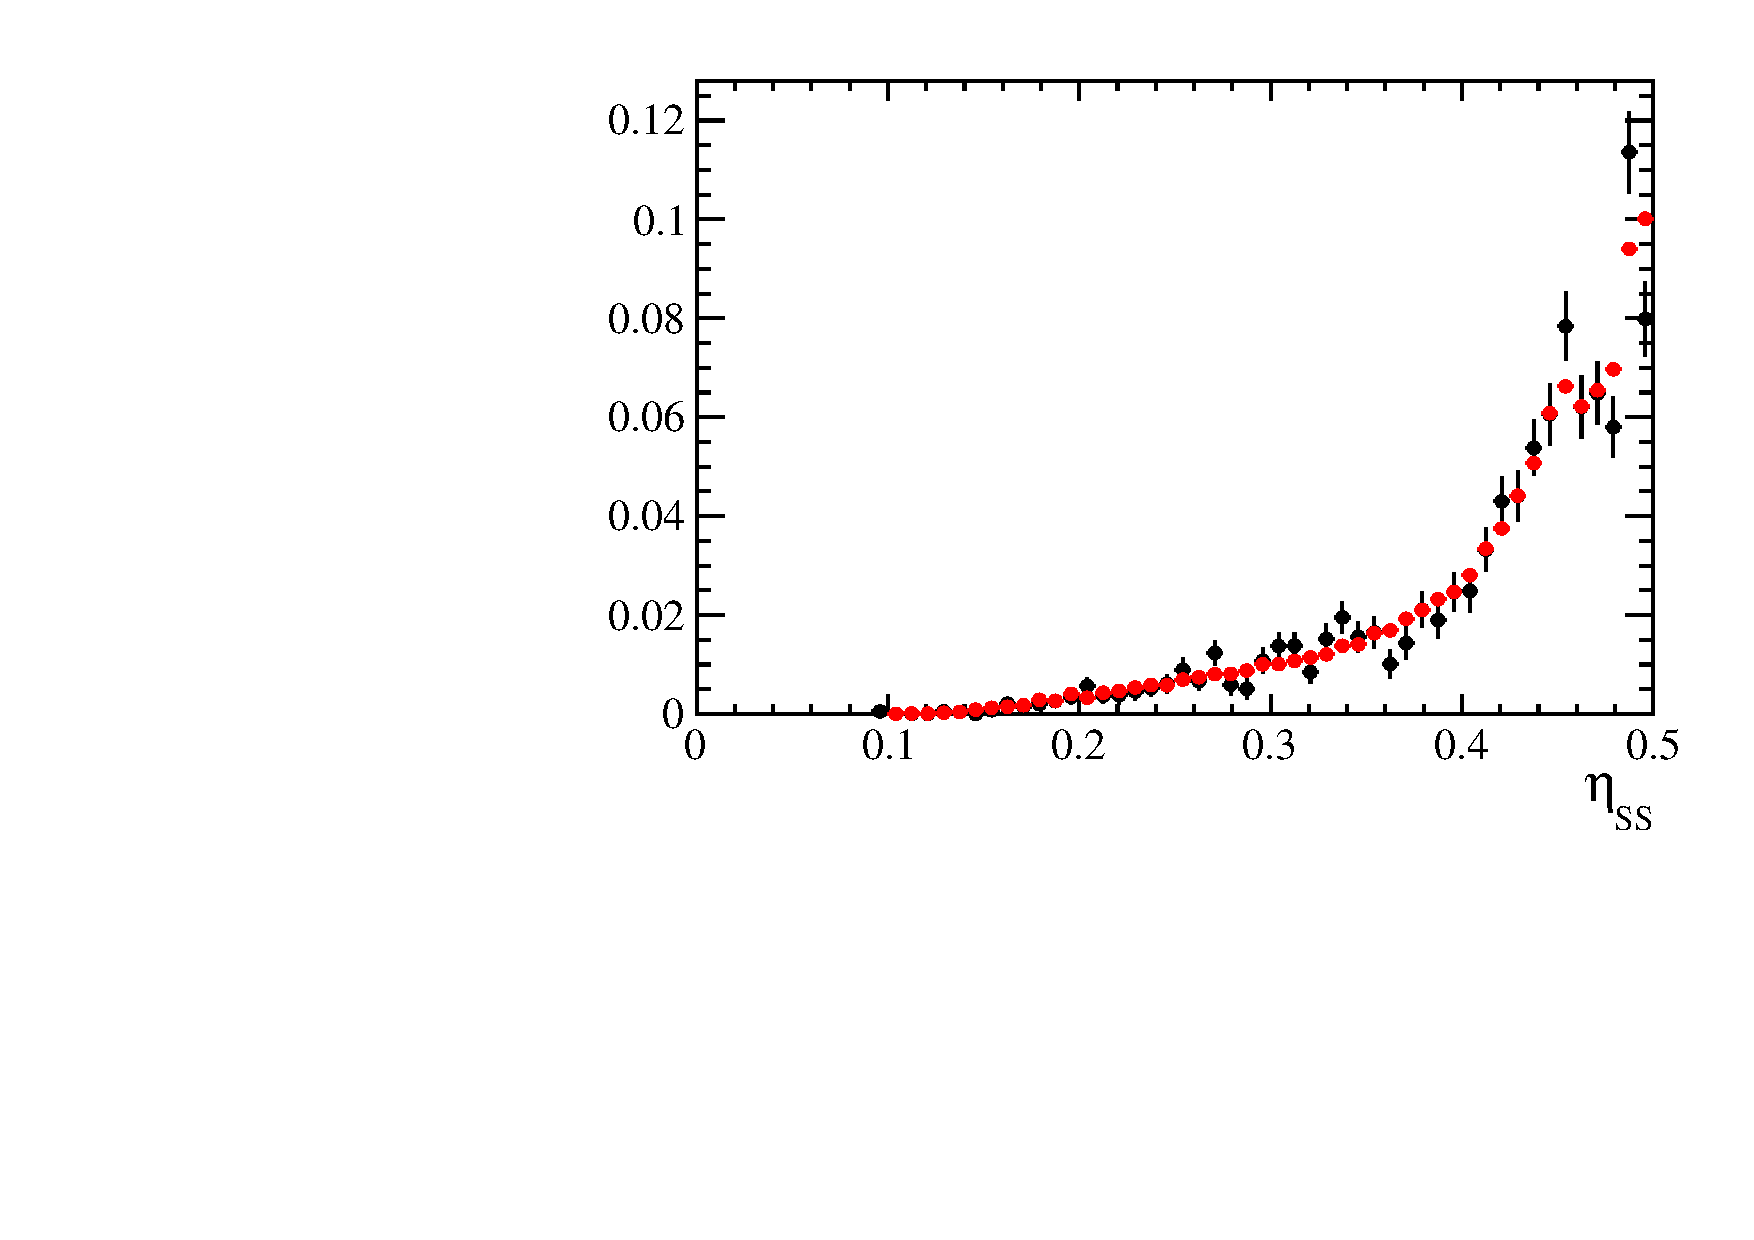
\includegraphics[height=7.cm,width=0.49\textwidth]{figs/Tagging/w_SS.pdf}
\caption{Distributions of the predicted mistag $\eta$ for the OS combination (left) and the SS kaon tagger (right) 
for signal candidates in the $\Bs\to\Ds\kaon\pion\pion$ (black) and $\Bs\to\Ds\pion\pion\pion$ (red) data samples. 
The signal distributions are obtained using sWeights, the procedure is described in Sec. \ref{subsec: sWegihts}.}
\label{fig:w_data_comparison}
\end{figure}


\begin{figure}[h]
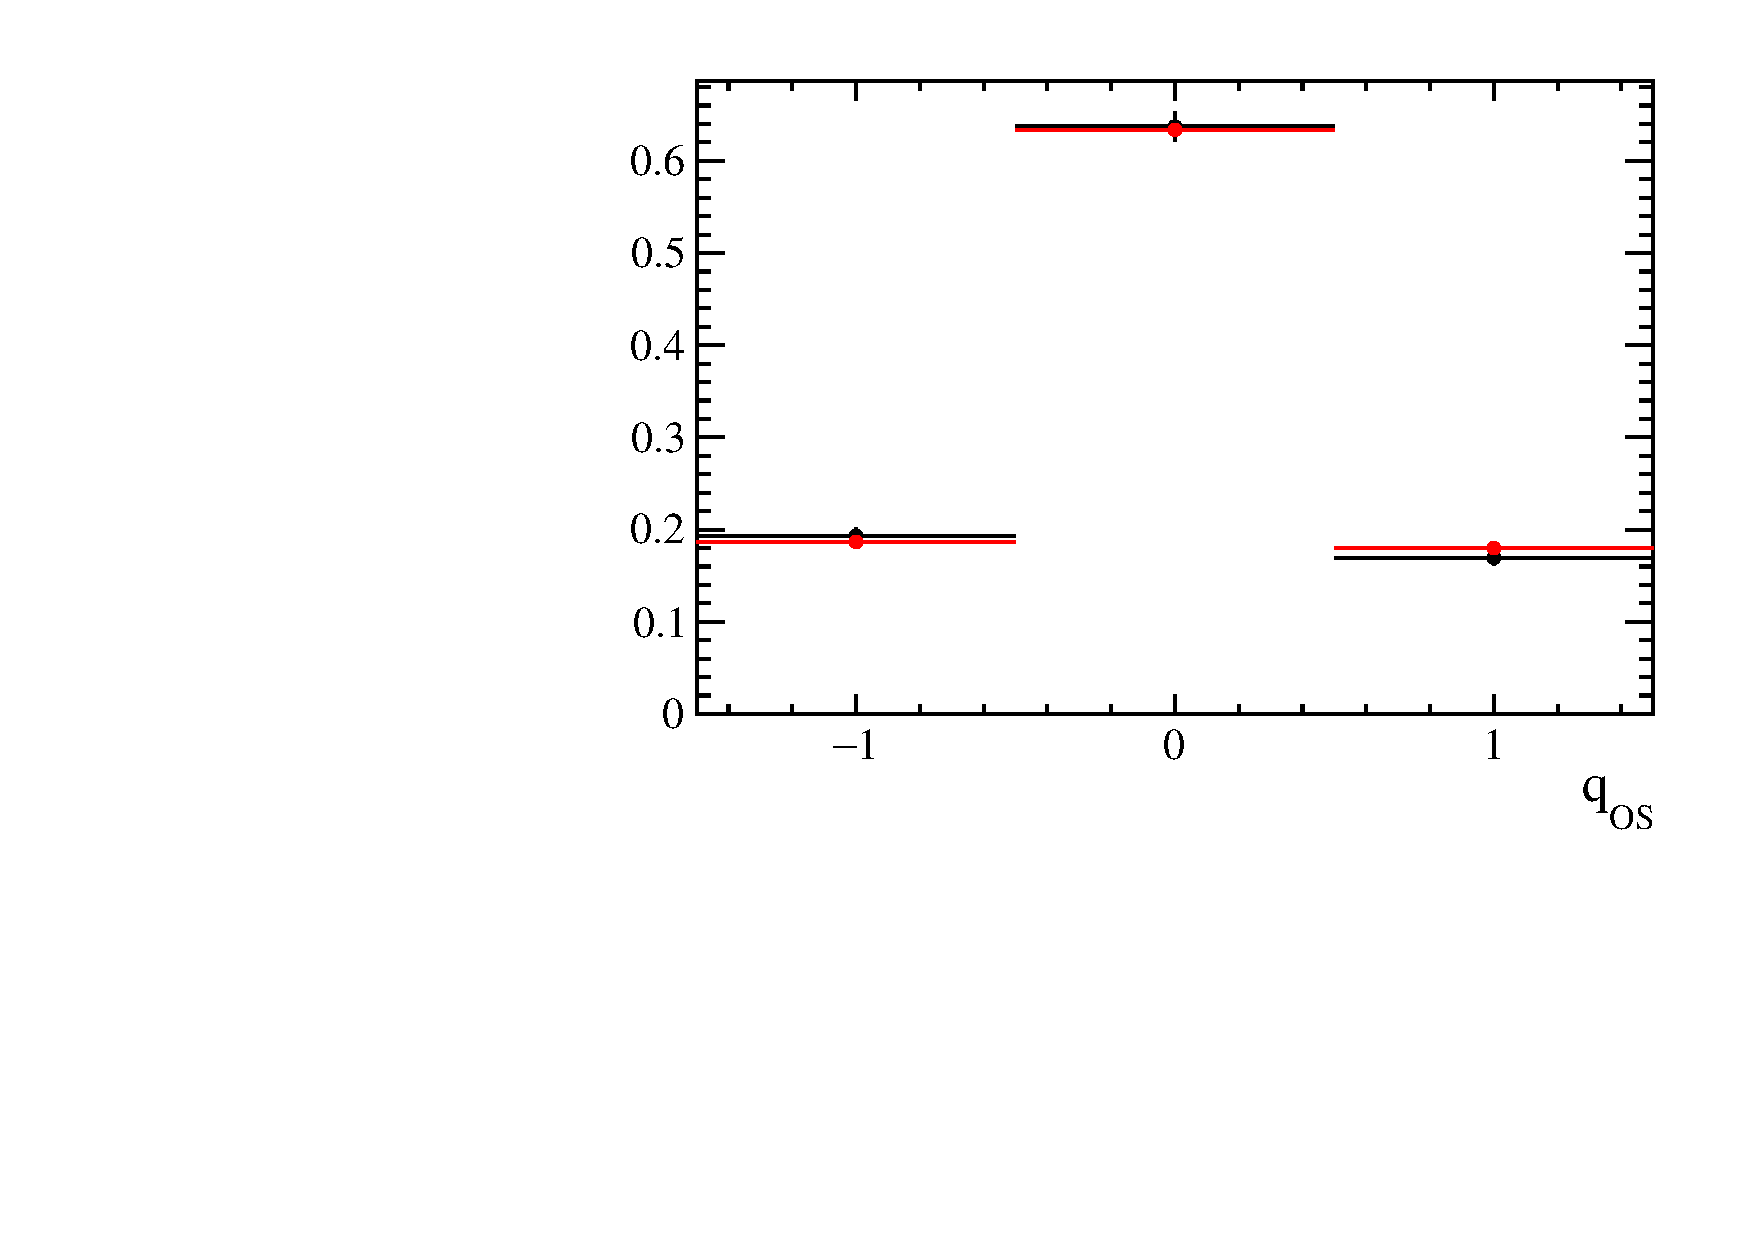
\includegraphics[height=7.cm,width=0.49\textwidth]{figs/Tagging/qOS.pdf}
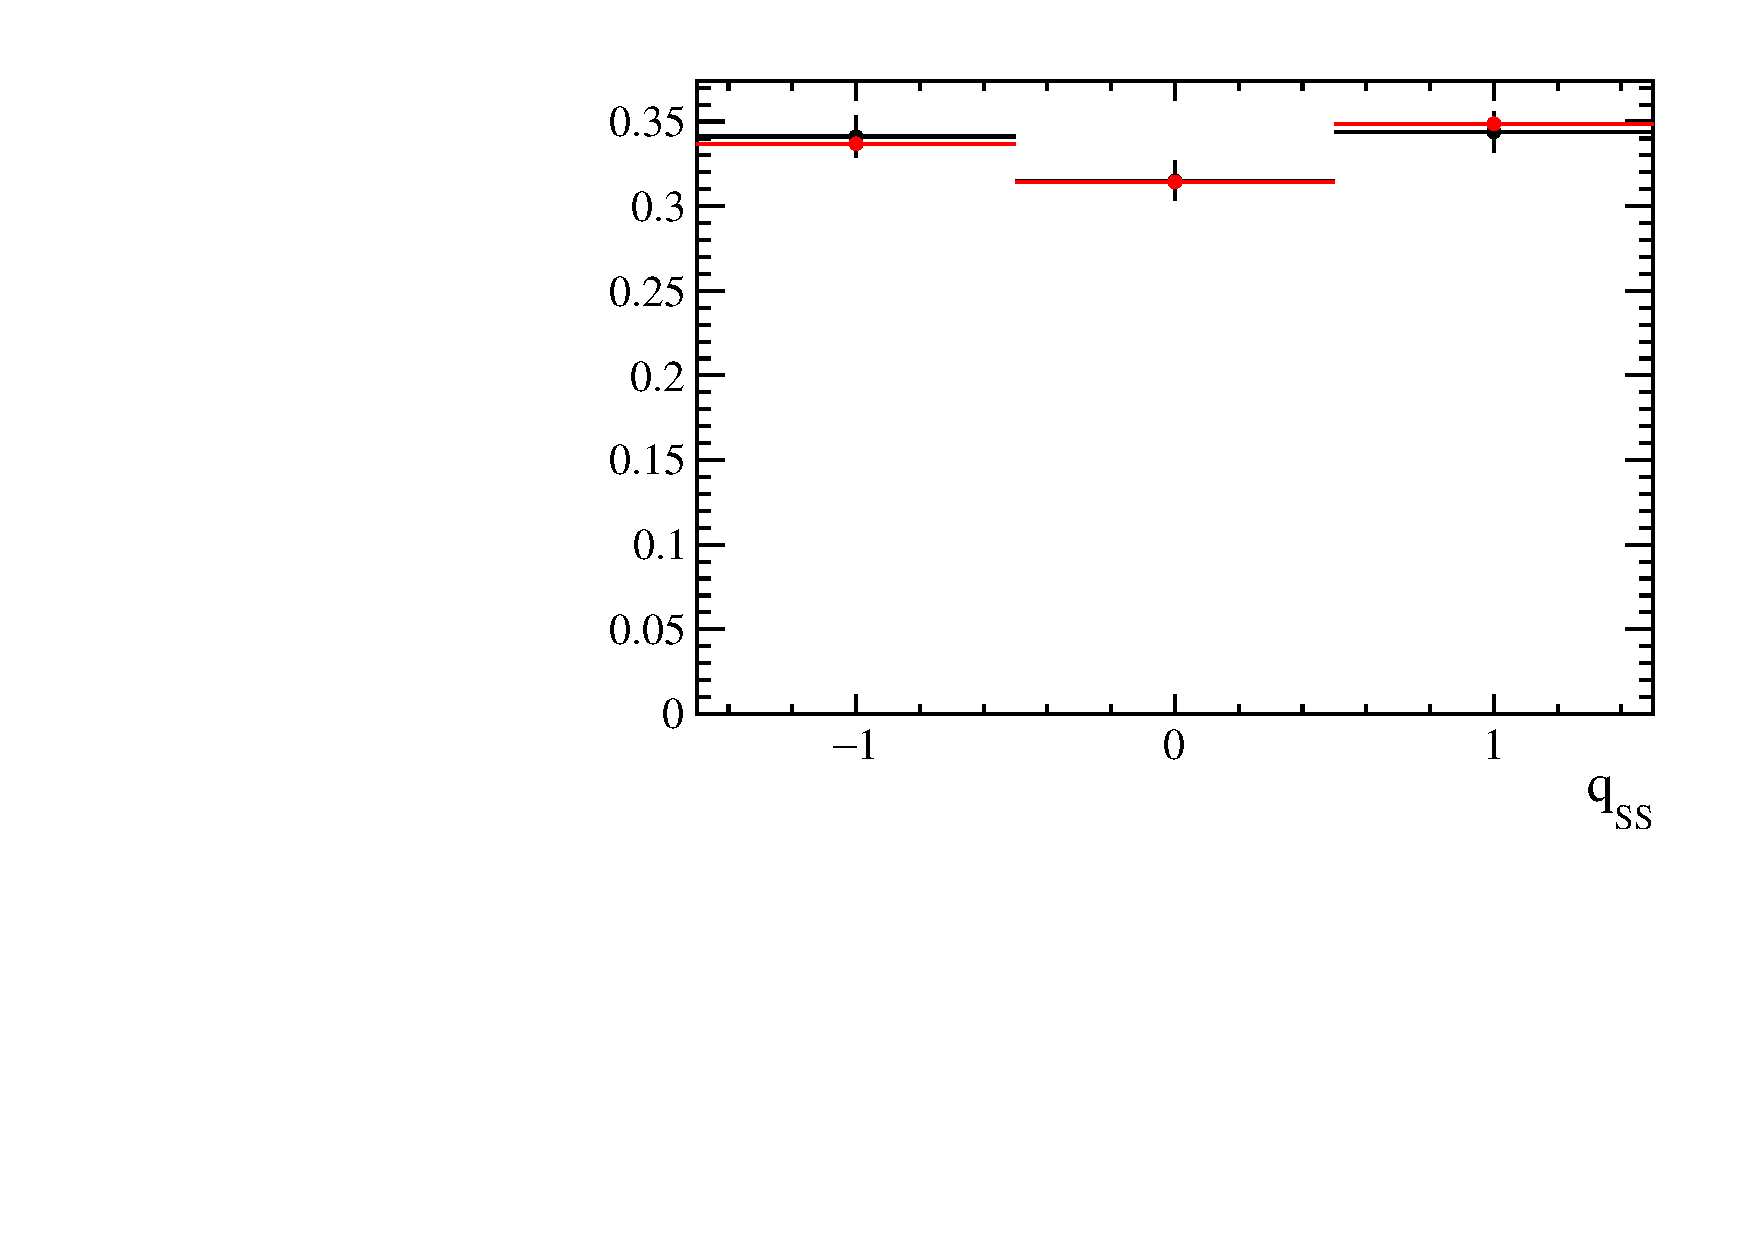
\includegraphics[height=7.cm,width=0.49\textwidth]{figs/Tagging/q_SS.pdf}
\caption{Distributions of the tagging decision from the OS combination (left) and the SS kaon tagger (right) for signal candidates in the $\Bs\to\Ds\kaon\pion\pion$ (black) and $\Bs\to\Ds\pion\pion\pion$ (red) data samples. 
The signal distributions are obtained using sWeights, the procedure is described in Sec. \ref{subsec: sWegihts}.}
\label{fig:w_data_comparison}
\end{figure}


\begin{figure}[h]
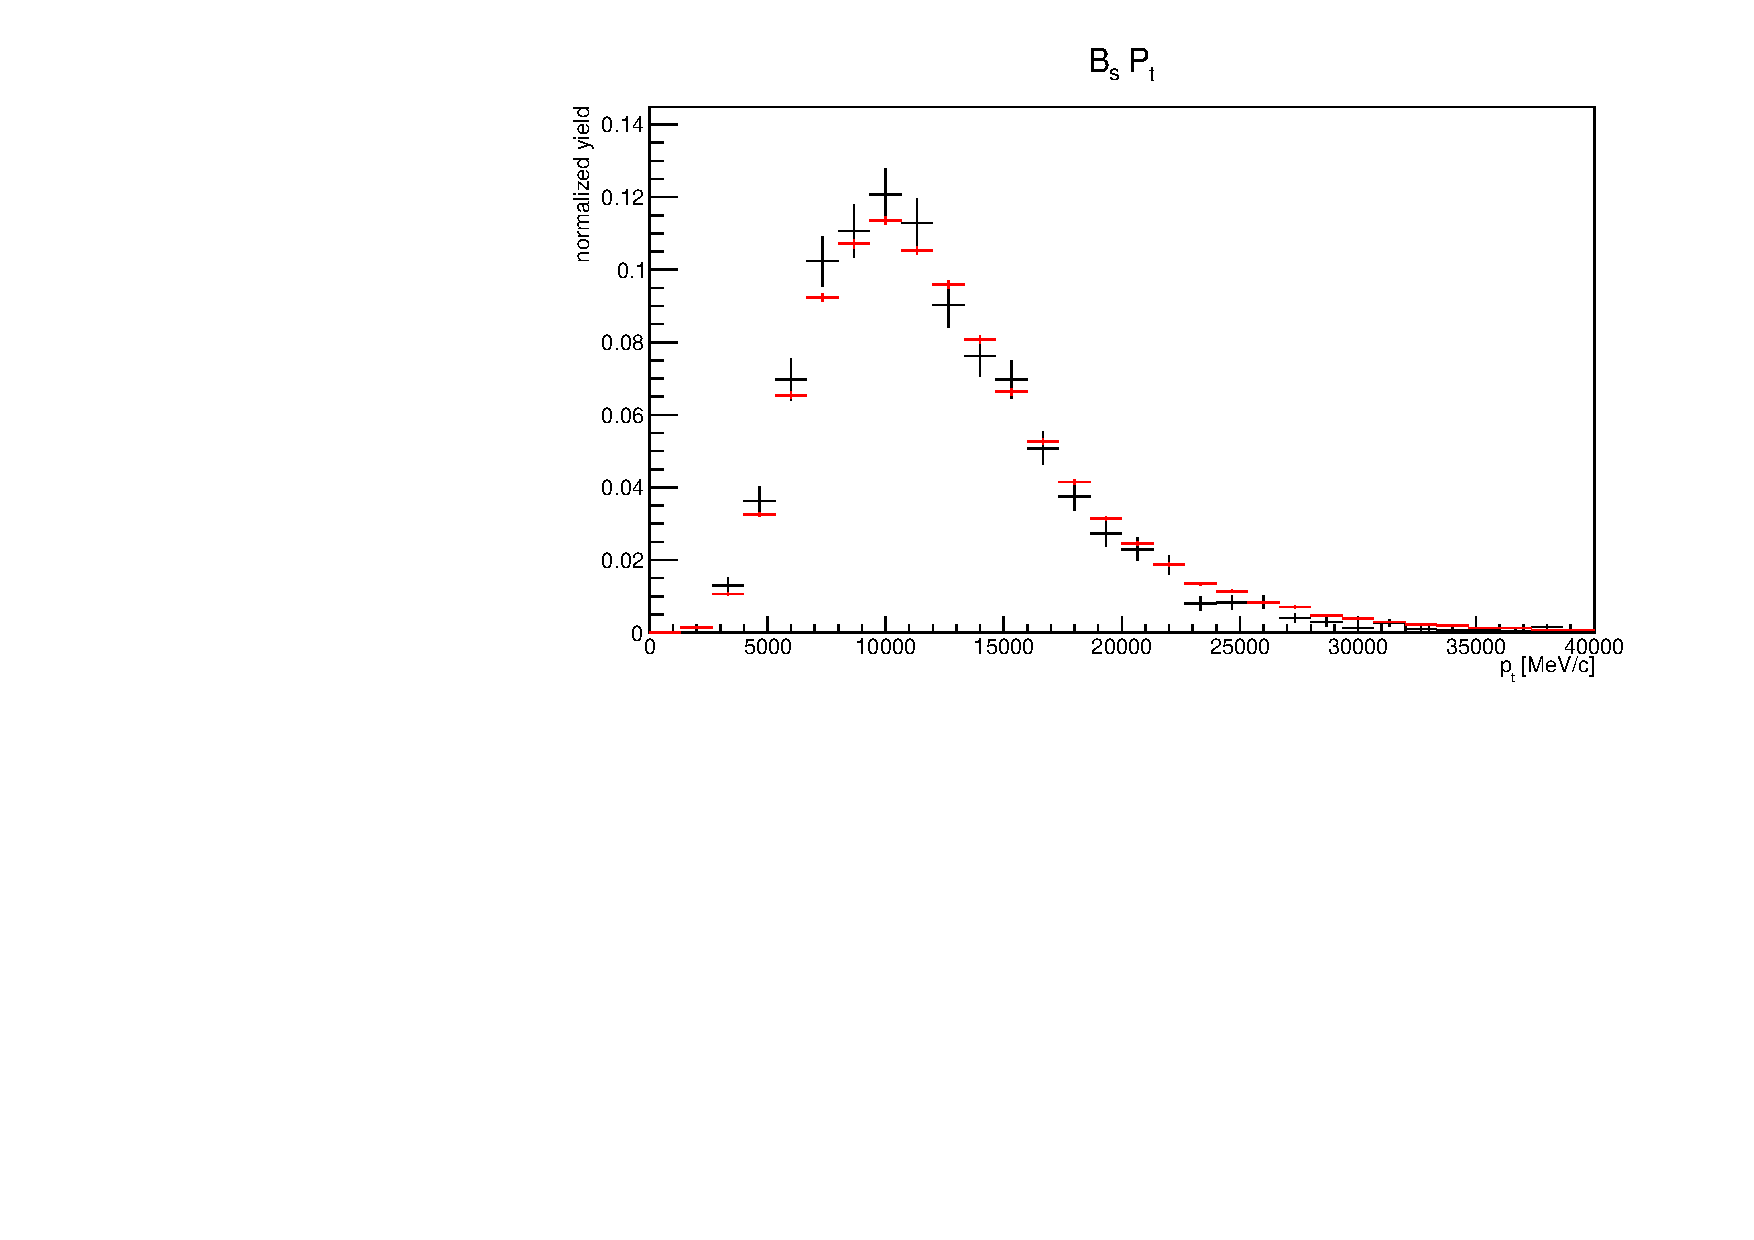
\includegraphics[height=7.cm,width=0.49\textwidth]{figs/Tagging/Bs_Pt_comparison.pdf}
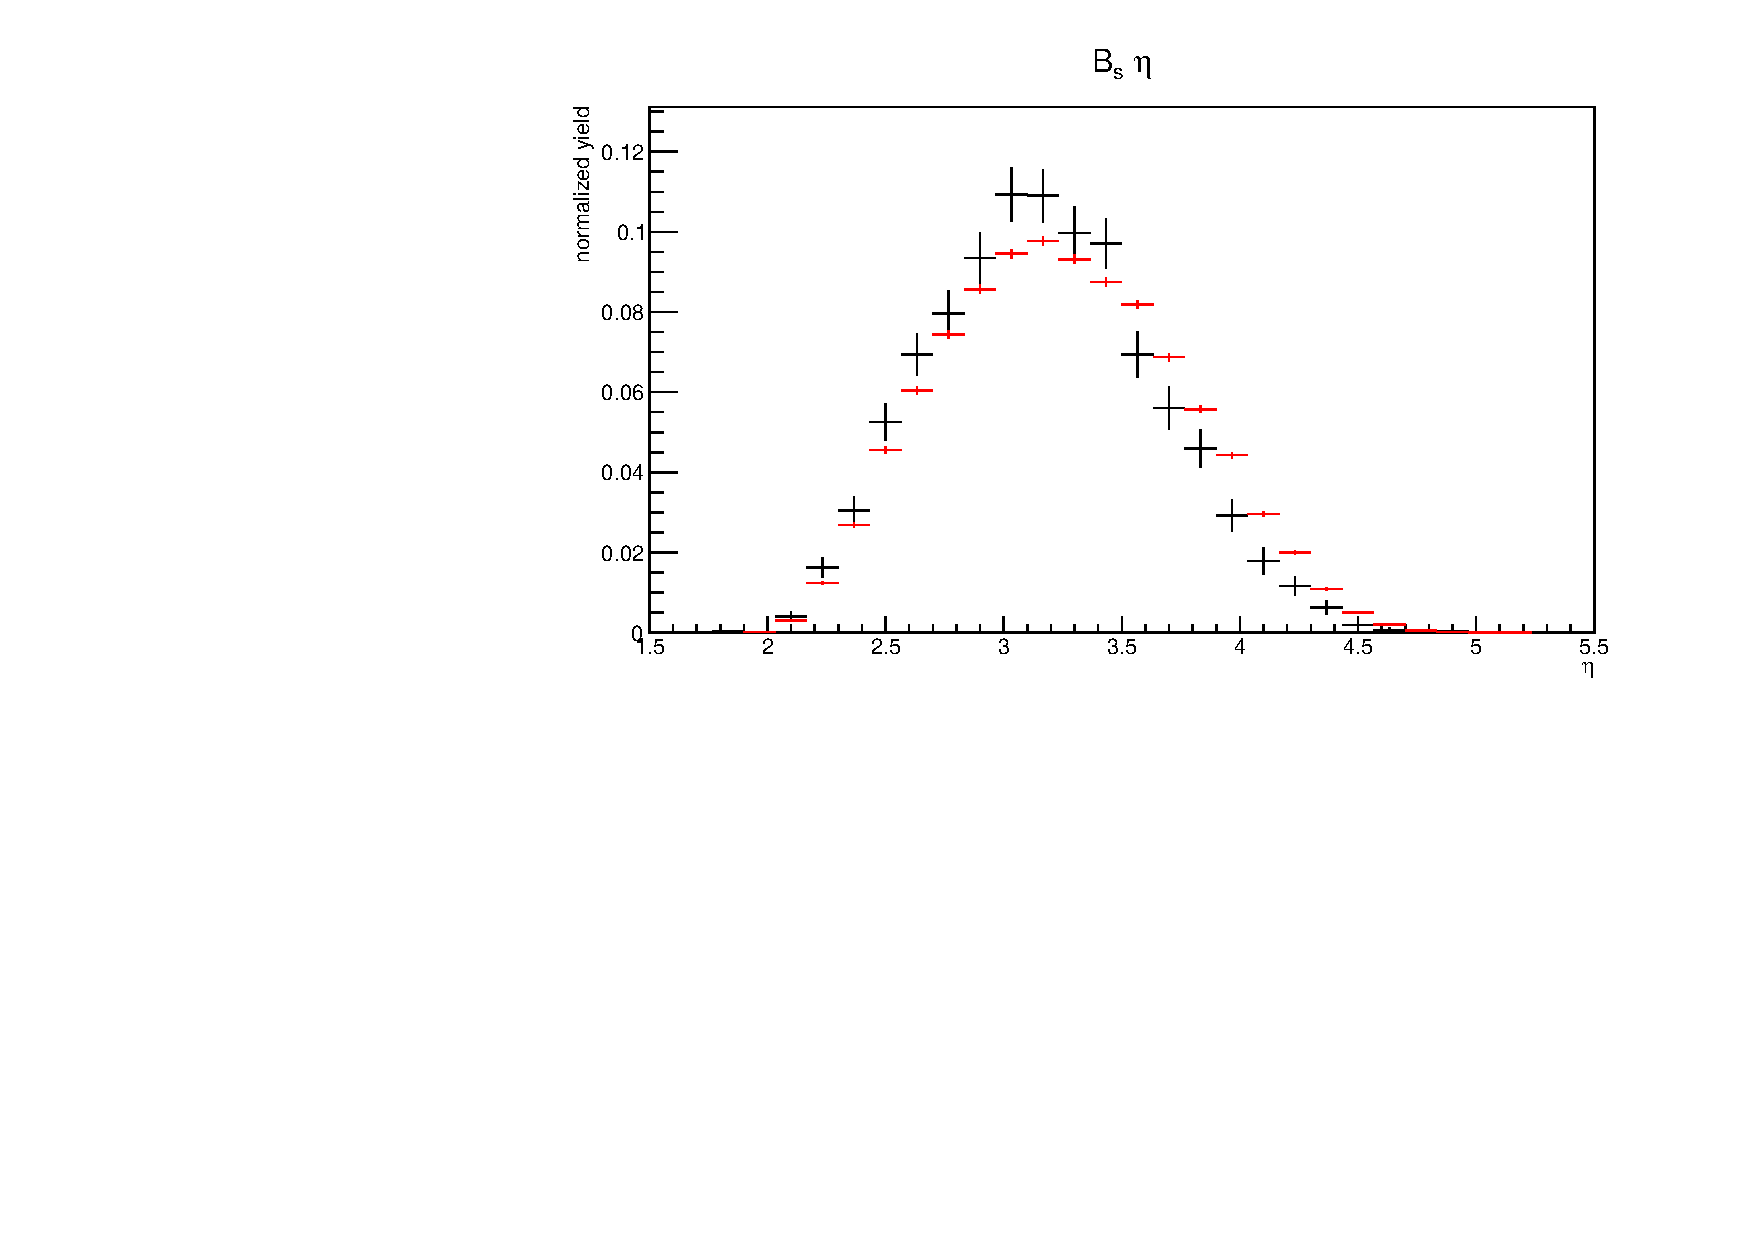
\includegraphics[height=7.cm,width=0.49\textwidth]{figs/Tagging/Bs_eta_comparison.pdf}\\
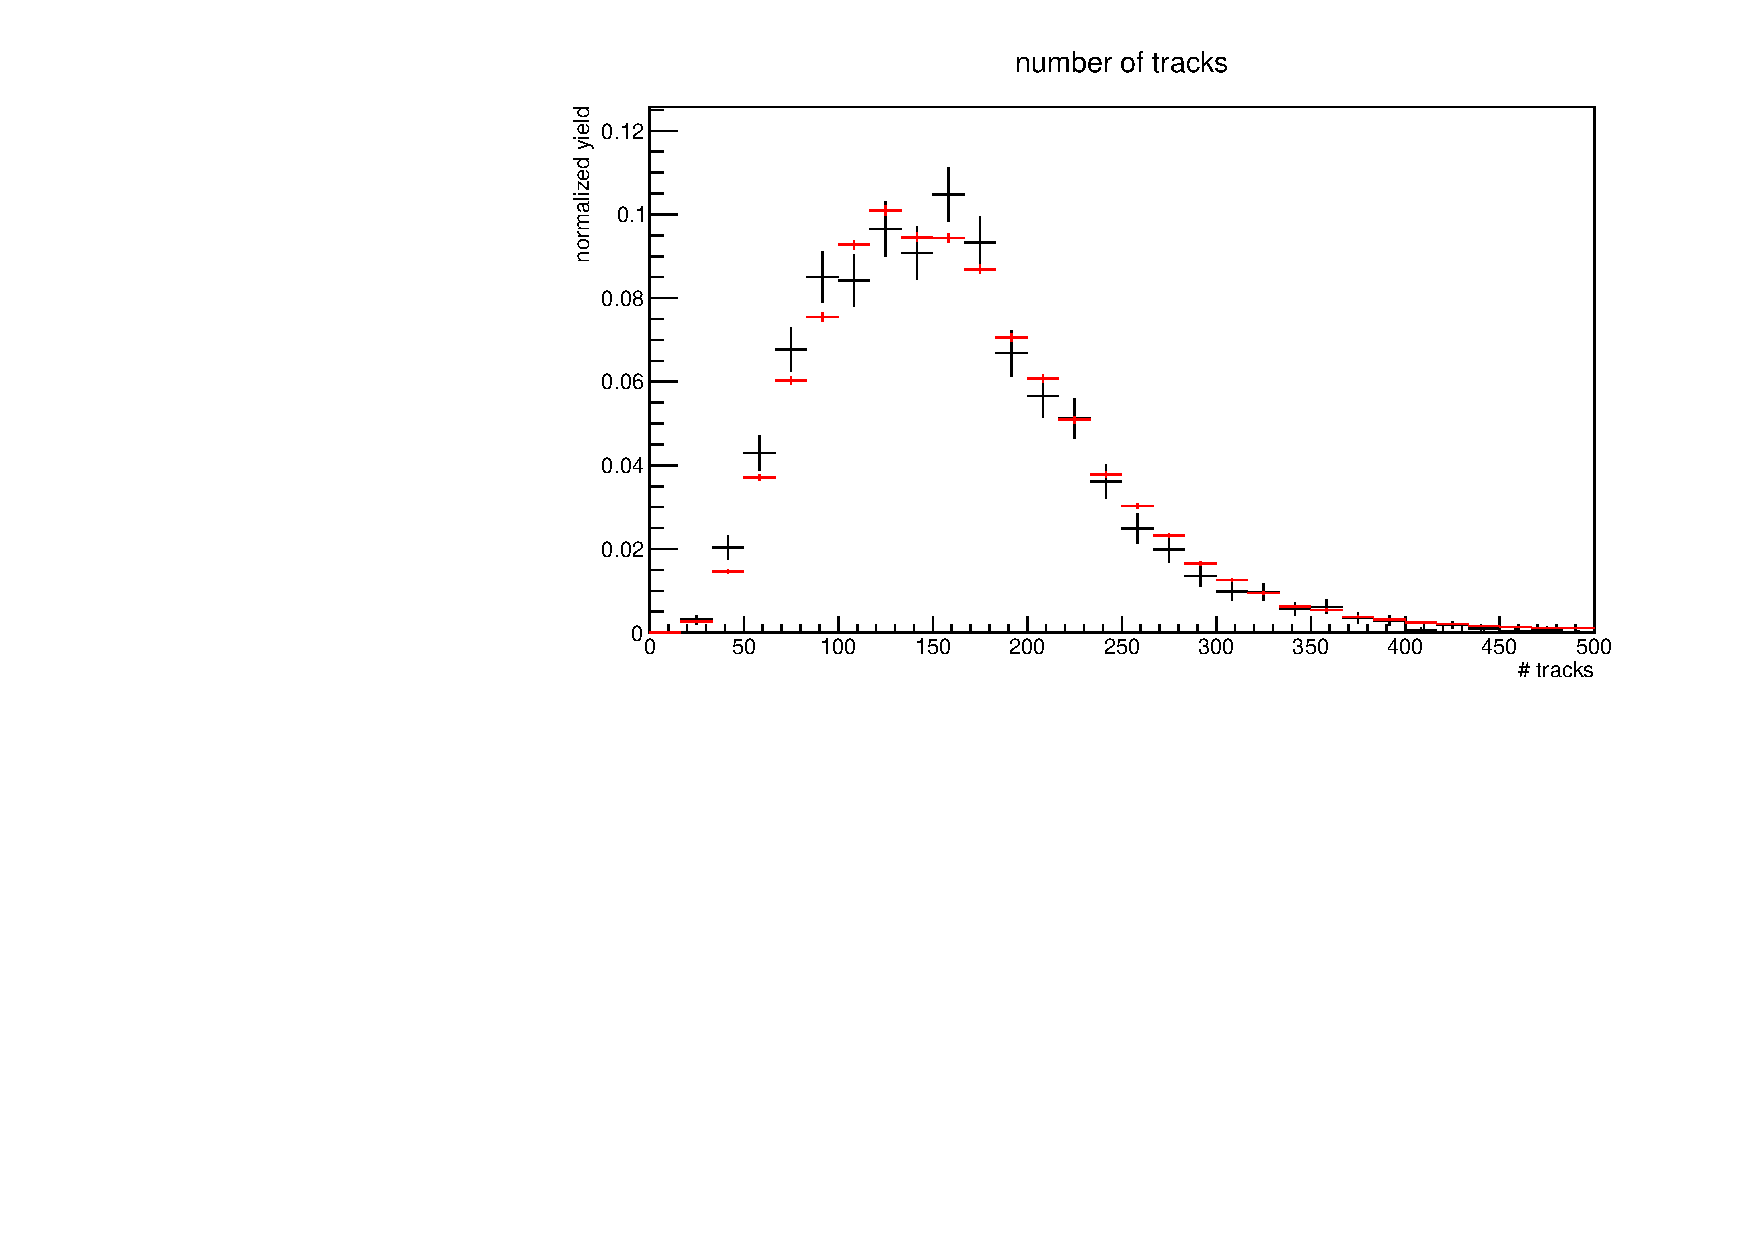
\includegraphics[height=7.cm,width=0.49\textwidth]{figs/Tagging/nTracks_comparison.pdf}
\caption{Distributions of the transverse momentum $\pt$ (top left), 
the pseudorapidity $\eta$ (top right) and the reconstructed number of tracks in the event (bottom left) for signal candidates in the $\Bs\to\Ds\kaon\pion\pion$ (black) and $\Bs\to\Ds\pion\pion\pion$ (red) data samples. 
The signal distributions are obtained using sWeights, the procedure is described in Sec. \ref{subsec: sWegihts}.}
\label{fig:w_data_comparison}
\end{figure}




\subsection{Combination of OS and SS taggers}
\label{subsec: TaggingCombination}


\begin{figure}[h]
\centering
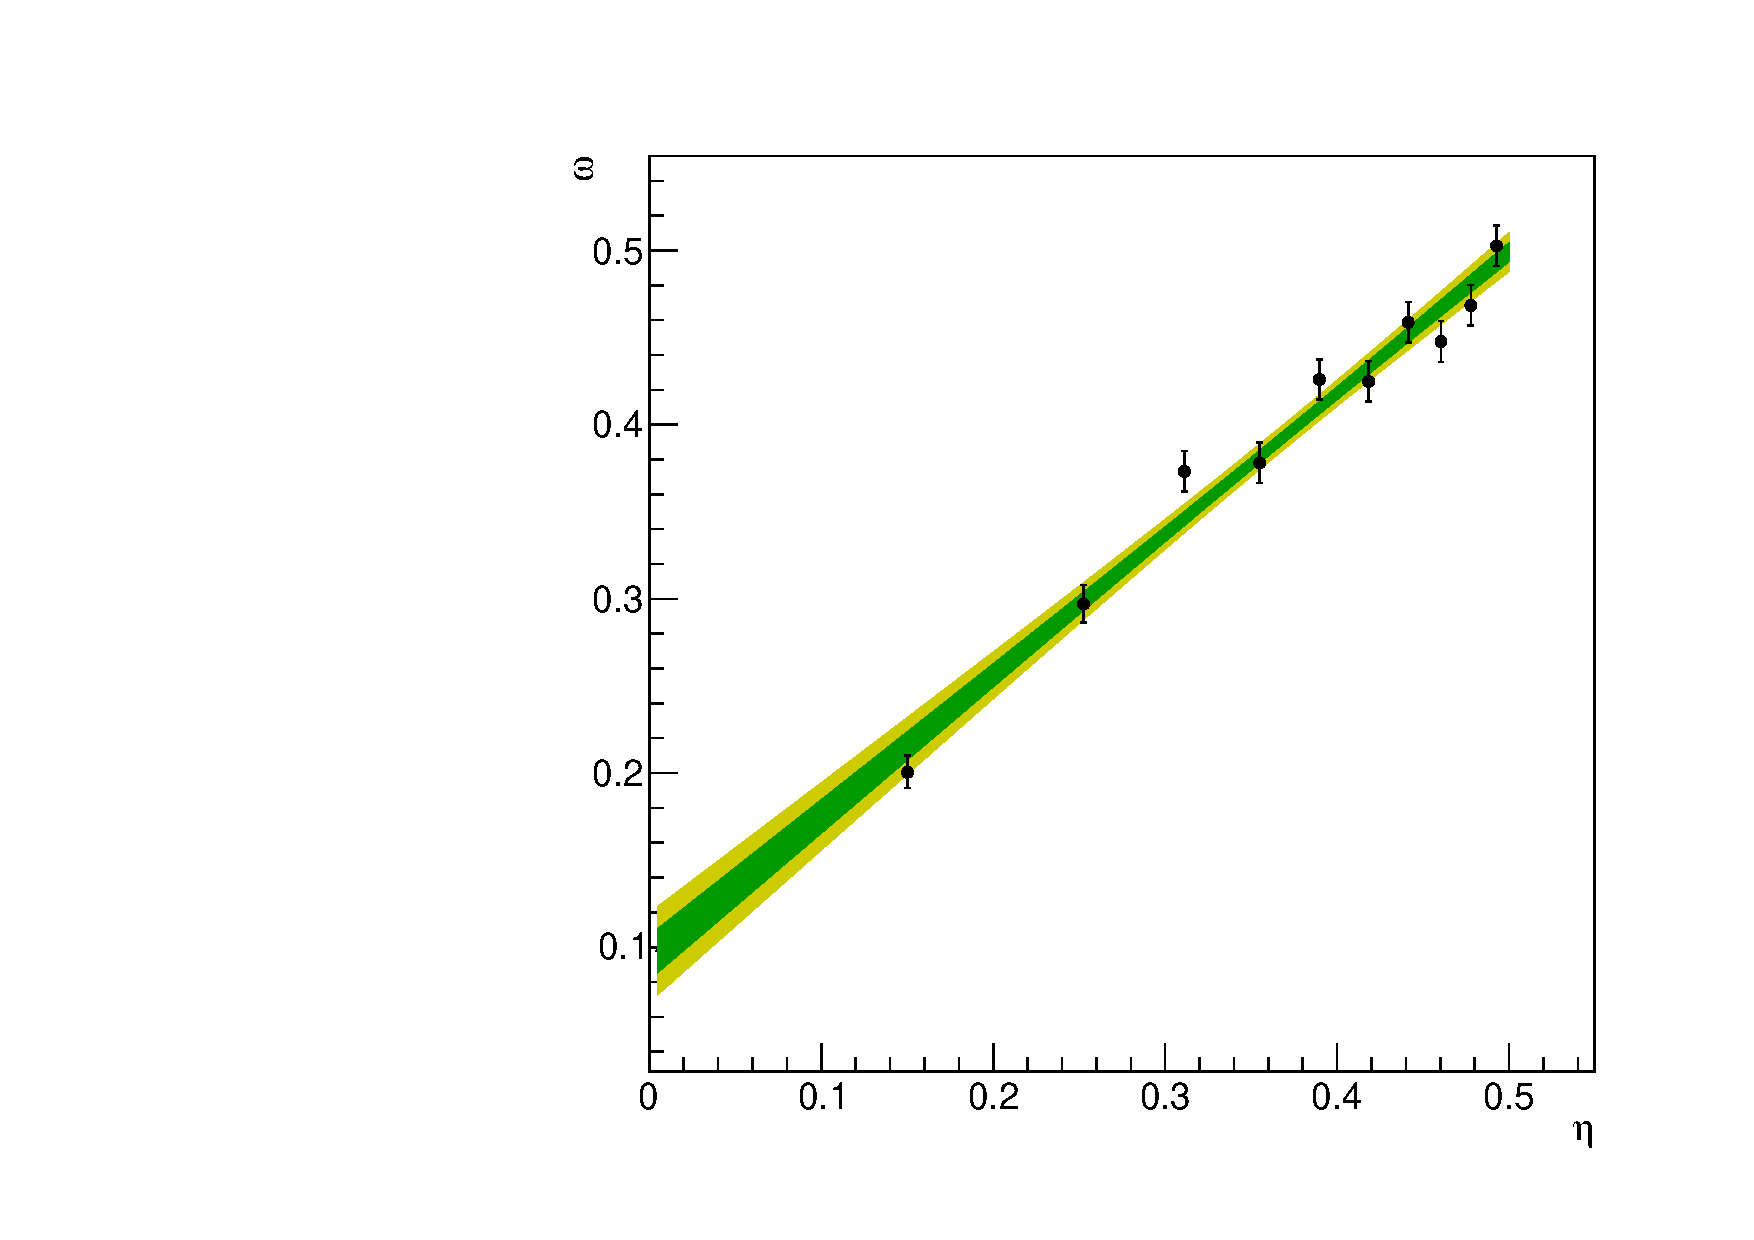
\includegraphics[height=7.4cm,width=0.7\textwidth]{figs/Tagging/TaggingCombinationCalibration.pdf}
\caption{Distribution of the predicted combined mistag probablity $\eta$ versus the observed mistag $\omega$ $\Bs\to\Ds\pion\pion\pion$ signal candidates. 
The fit with a linear polynomial, used to determine $p_{0}$ and $p_{1}$ is overlaid.}
\label{fig:TaggingCombinationCalibration}
\end{figure}
